\subsection{Harmoniske svingninger}\label{teori: Harmoniske svingninger}
En oscillerende bevægelse er en bevægelse hvor et objekt, som bliver flyttet fra sit hvilested og sluppet vil bevæge sig tilbage mod sit hvilested, hvor det vil bevæge sig forbi sit hvilested for igen at foretage gentagelser af netop dette for til slut at ende på sit hvilested igen. Dette kan eksempelvis ses hos penduler og masser bundet til fjedre.
\\

\begin{wrapfigure}{r}{0.3\textwidth}
\centering
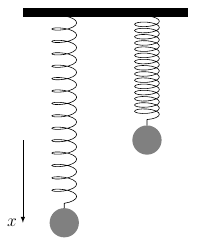
\includegraphics[scale=1]{Billeder/fjeder}
\caption{Fjeder med lod \label{fig:fjeder}}
\end{wrapfigure} 

Eksemplet der vil blive betragtet i dette kapitel er oscillerende bevægelse, der er hensigtsmæssig i forhold til at forstå IR-spektroskopier. Vi vil se på en masse der er bundet til en fjeder. se figur \ref{fig:fjeder}.

Med udgangspunkt i figur \ref{fig:fjeder} vil vi se på en masse der i den ene ende er fastgjort til noget stationært og i den anden ende er fastgjort til en kugle med en masse. Når kuglen ikke påvirkes af andre ydre kræfter en tyngdekraften vil kuglen opnå en hviletilstand hvor fjederkraften er lige så stor som tyngdekraften. Vi sætter denne hviletilstand til $x_0=0$. Når vi så begynder at påvirke system med en ydre kraft ved f.eks. at hive i kuglen vil fjederen svare tilbage ved at trække endnu hårdere i kuglen. Hvis vi op som den positive retning vil vi på figur \ref{fig:fjeder} have flyttet kuglen en afstand $-x$ væk fra sin hvileposition vil fjederkraften givet ved Hookes lov, der blev beskrevet i \ref{Hookes} være givet ved $F_x=-k \cdot x$. Hvor F er fjedekraften, k er fjederkonstanten for den givne fjeder og x er afstanden flyttet fra hvilepositionen $x_0$